\section{Numerical Results}
\label{sec:numres}
With the mathematical model now fully established, the implementation of this model is documented in Section \ref{subsec:impl}. From here Sections \ref{subsec:vv} verifies the model against exact dispersion relations for multiple modes in rectangular waveguides. Section \ref{subsec:circ_guides} performs an analysis of Dispersion characteristics in circular waveguides and addresses the advantages of using FEA for this task. Finally, Section \ref{subsec:rid_guides} compares the dispersion characteristics of the rectangular and ridged rectangular waveguides for multiple modes and discusses practical applications of ridged waveguides.

\subsection{Implementation}
\label{subsec:impl}
meshing

code implementation

\subsection{Verification and Validation}
\label{subsec:vv}

present data for 10,20,30 (maps,a nd data)
\begin{figure}[t!]
	\begin{subfigure}{\linewidth} %\make this subfigure take up 80% of a linewidth
		\centering
		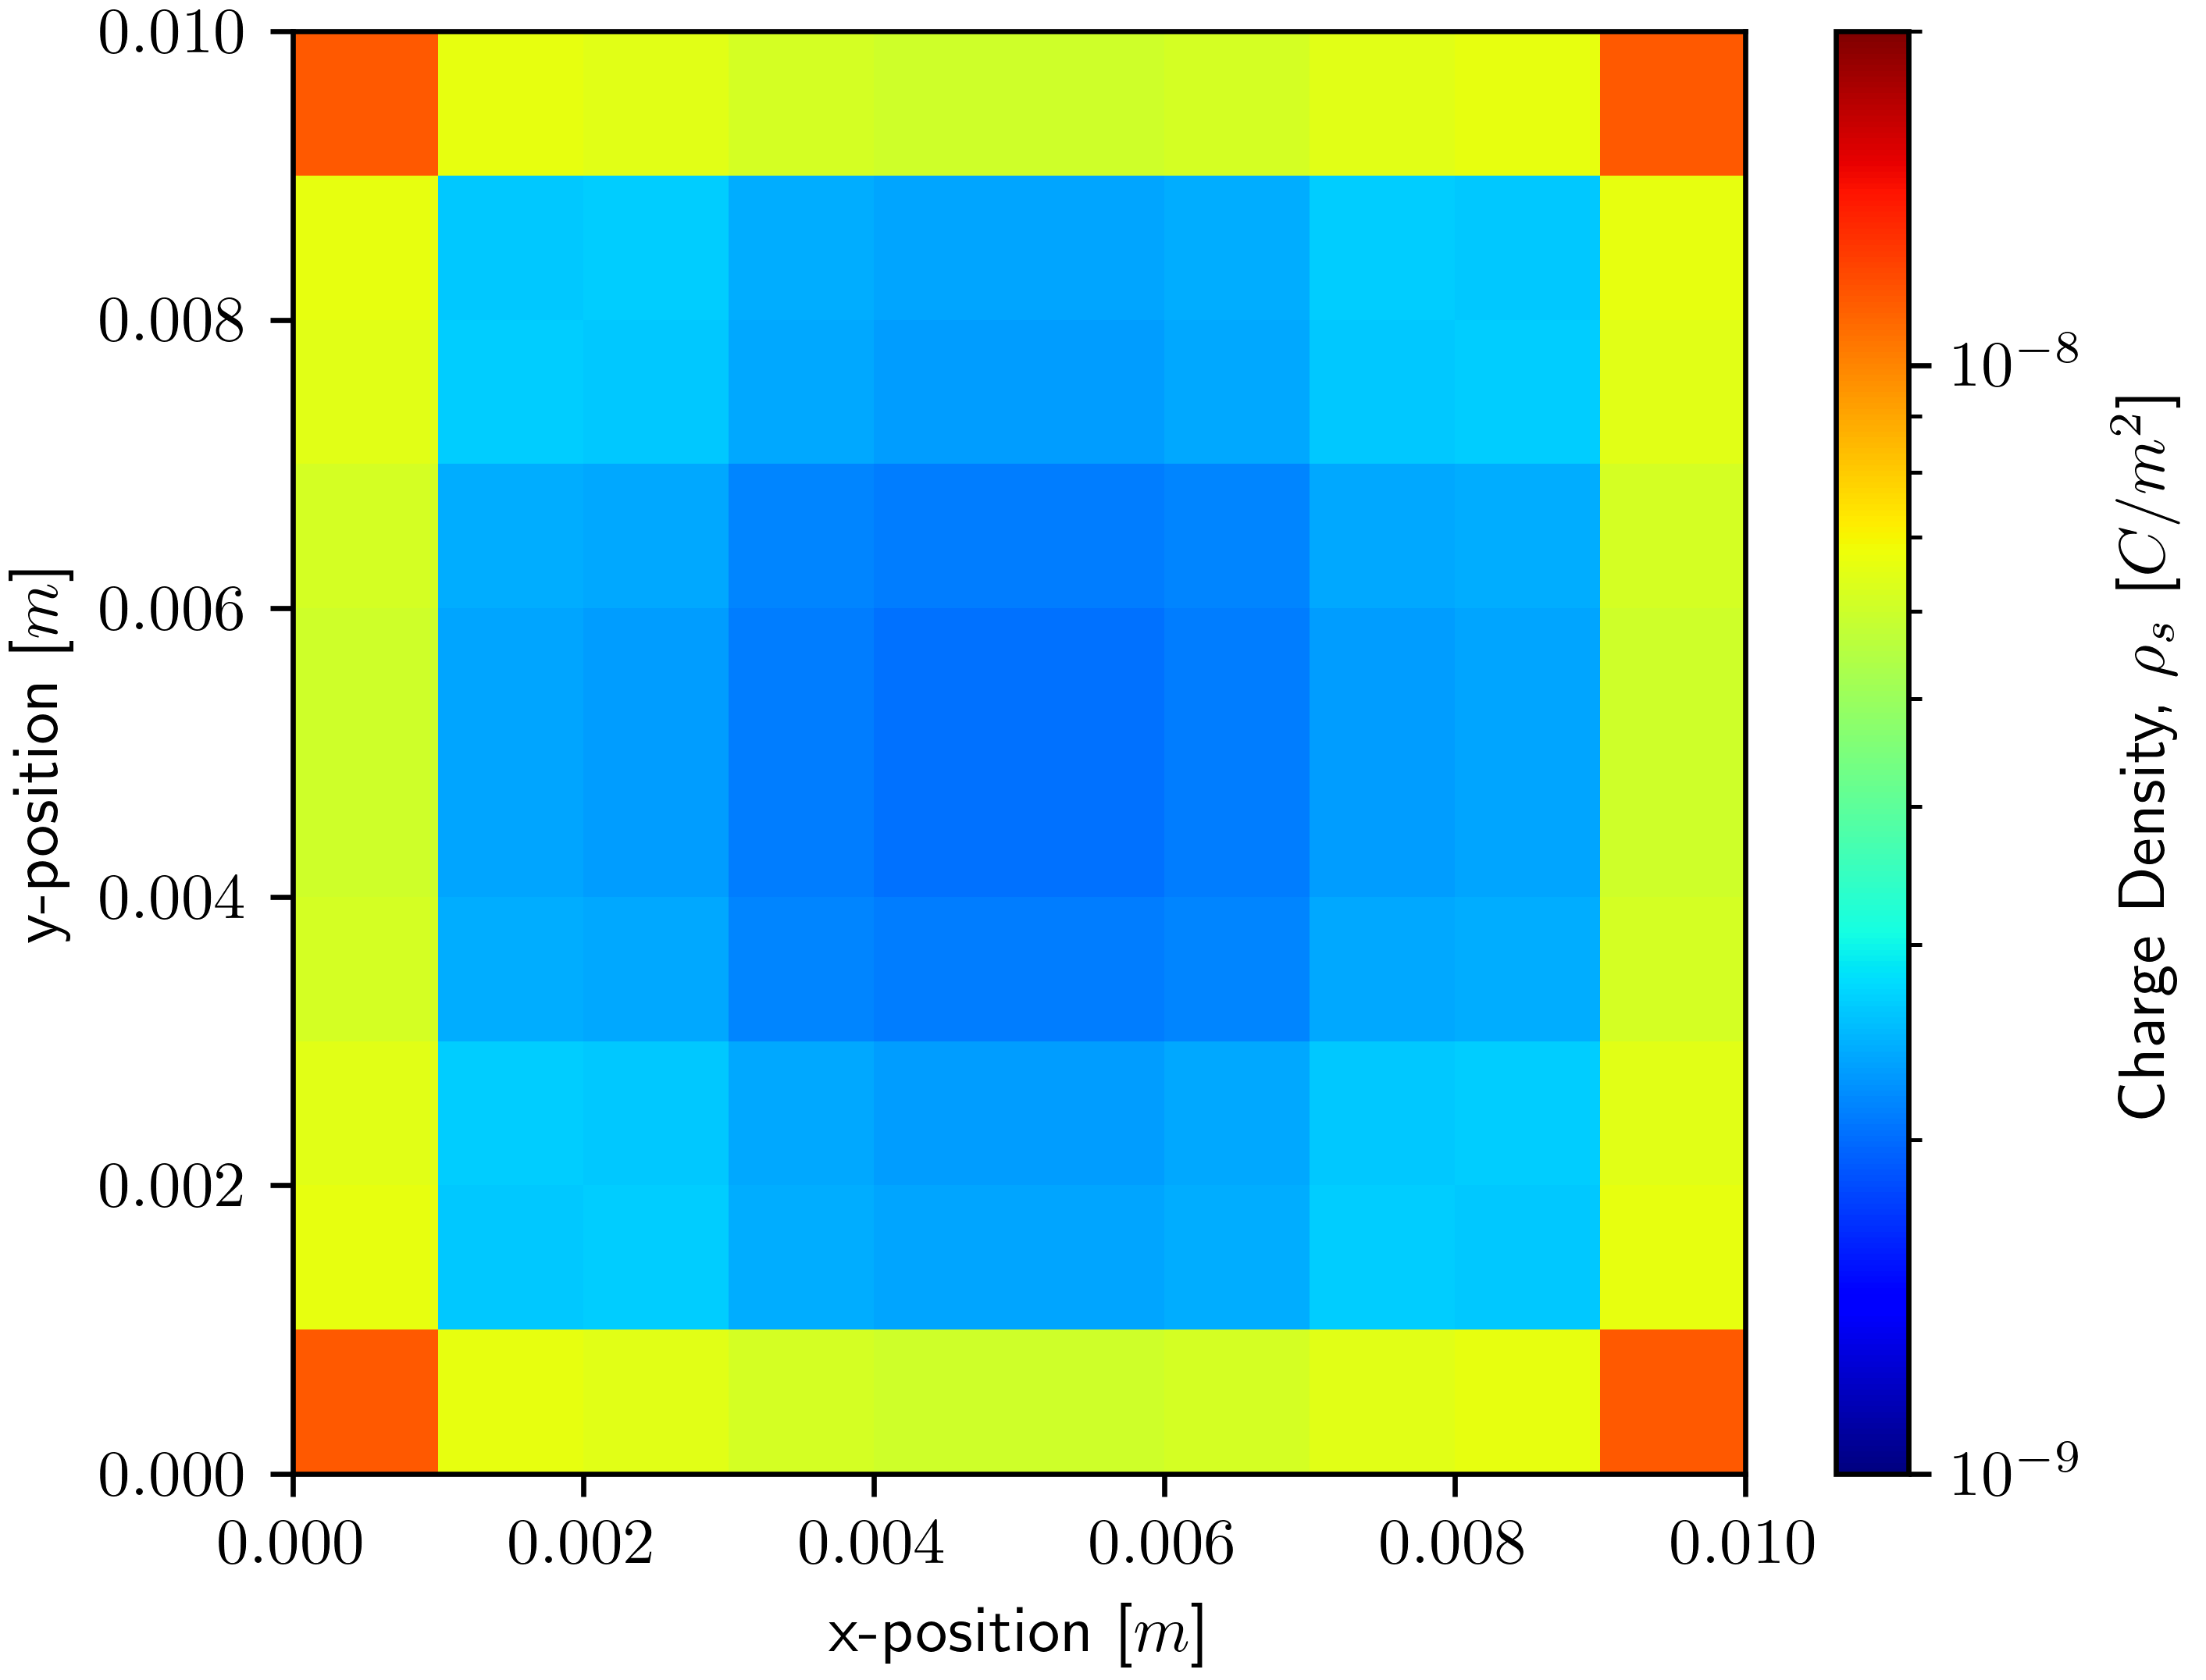
\includegraphics[width=\textwidth]{subd_10.png} %within this subfigure take up the entire textwidth (which was set by the linewidth command above)
		\caption{}
		\label{subfig:waveport1}
	\end{subfigure}
	\begin{subfigure}{\linewidth}
		\centering
		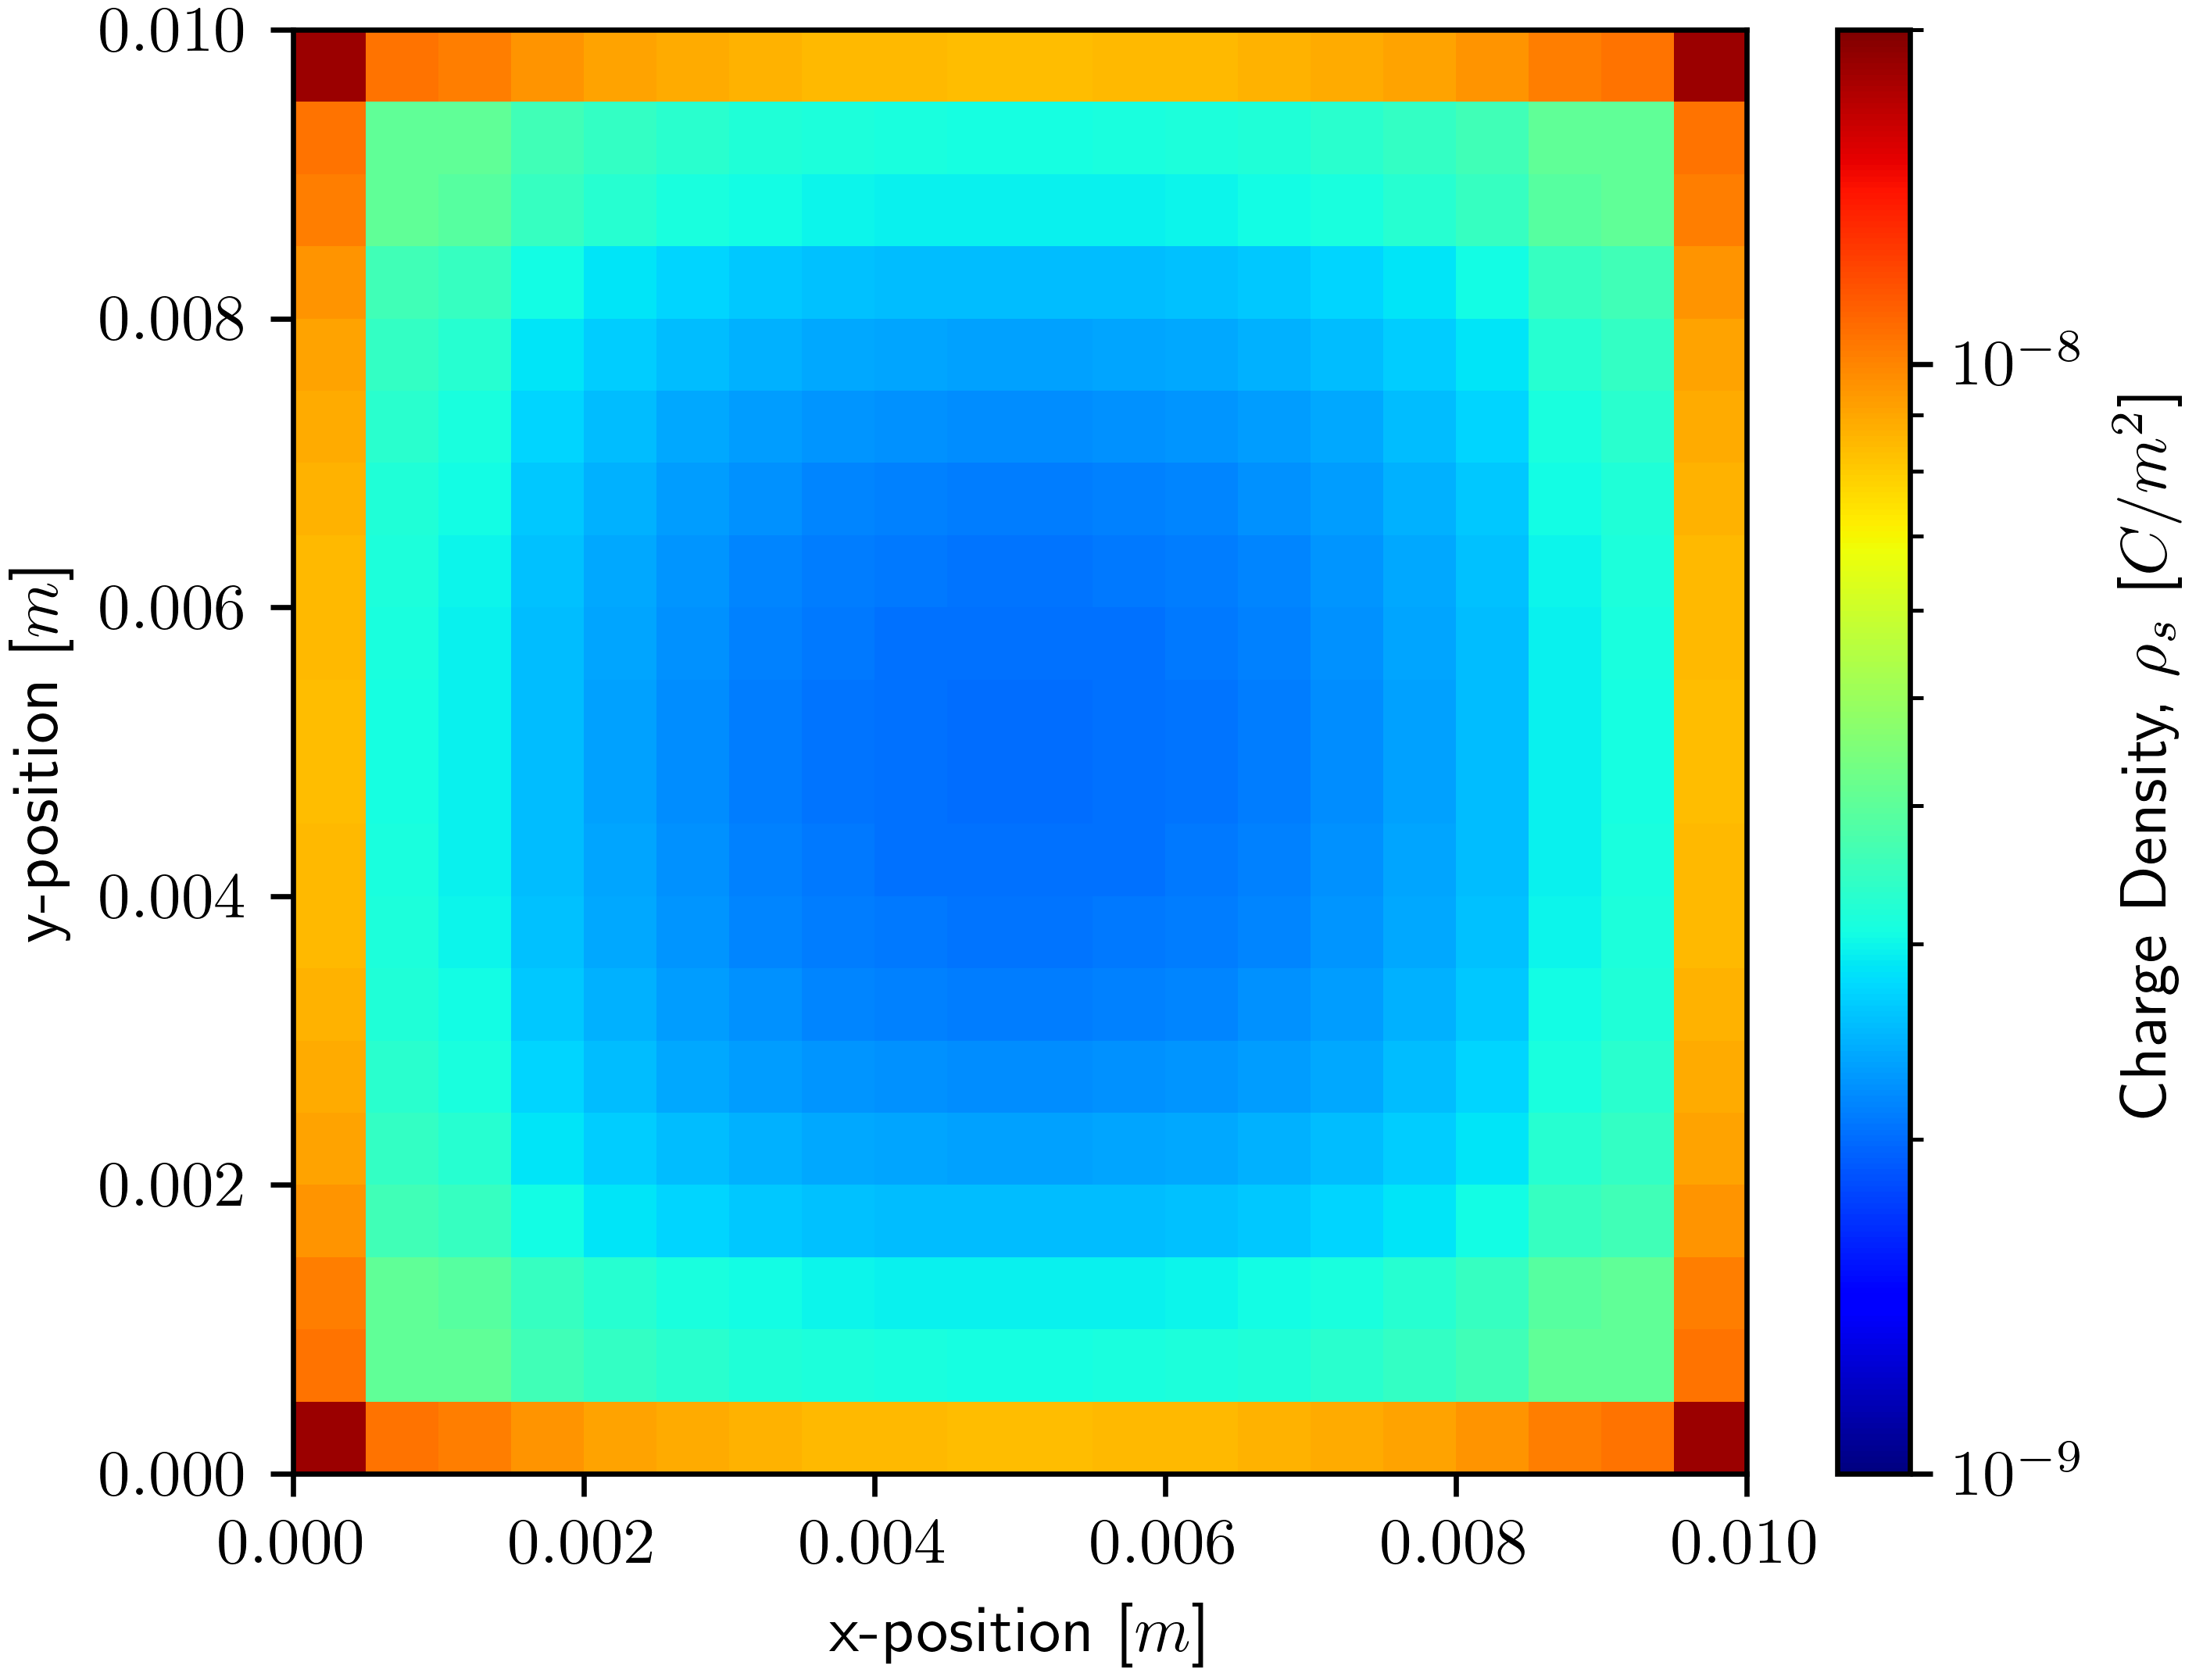
\includegraphics[width=\textwidth]{subd_20.png} %waveport2 is the name of the jpg file within the ./figures folder
		\caption{} %leave the caption blank, but you need the empty caption command for the (b) label to be made
		\label{subfig:waveport2}
	\end{subfigure}
	\begin{subfigure}{\linewidth}
		\centering
		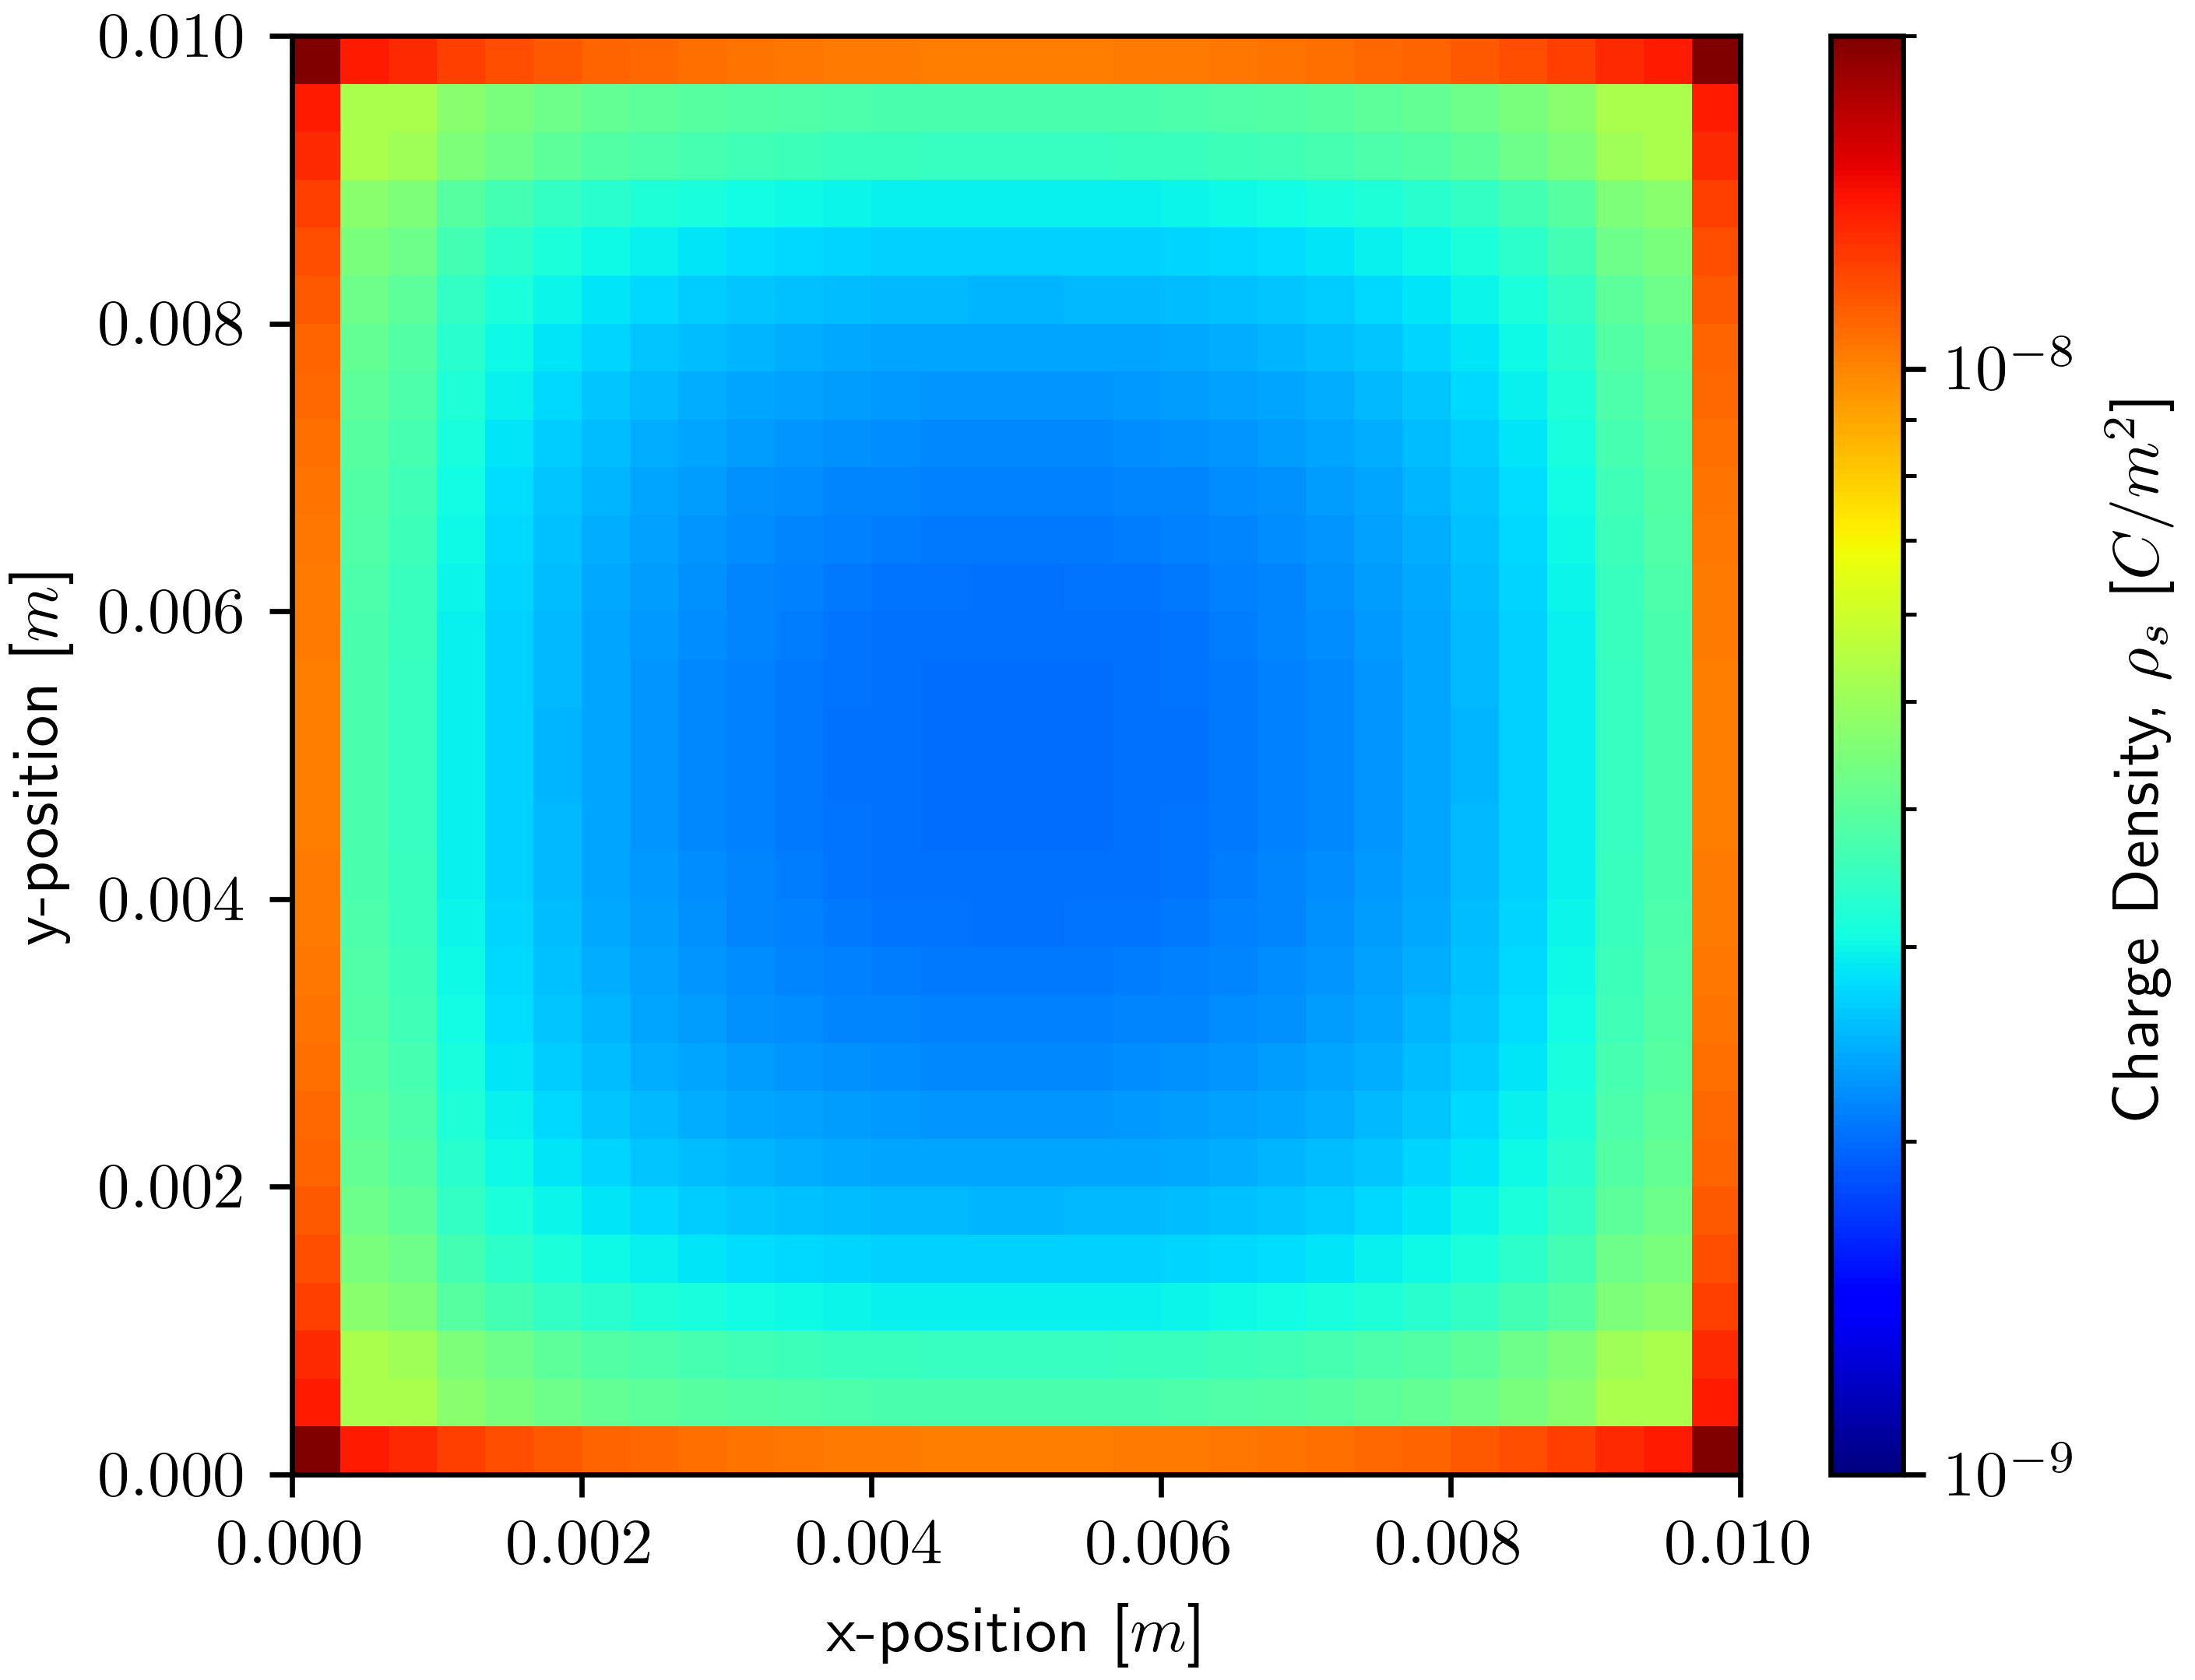
\includegraphics[width=\textwidth]{subd_30.png} %waveport2 is the name of the jpg file within the ./figures folder
		\caption{} %leave the caption blank, but you need the empty caption command for the (b) label to be made
		\label{subfig:waveport2}
	\end{subfigure}
	\caption{Use of wave ports to analyze a cylindrical cavity resonator. (a) The geometry analyzed and (b) the comparison of numerical and measured results (from \cite{jin2011theory}).}
	\label{fig:charge_d}
\end{figure}

\begin{tabular}{ |p{2cm}||p{1cm}|p{1cm}|p{1cm}|}
	\multicolumn{4}{c}{Table 1: Predicted Capacitances [pF]} \\
	\hline
	Method & $10\times10$ & $20\times20$ & $30\times30$ \\
	\hline
	Circular Element Approximation   & 0.397 &0.403 & 0.405\\
	\hline
	Exact Square Elements& 0.394& 0.401 & 0.403\\
	\hline
	Subdomain Collocation&0.399 & 0.403 & 0.405 \\
	\hline
   \end{tabular}

random walk solutions

show agreement


\subsection{Convergence Study}
\label{subsec:cs}
 plot and talk
 \begin{figure}[t!]  
	\centering
	%the command within the [] sets the width of the figure, stability-condition is the jpg name
	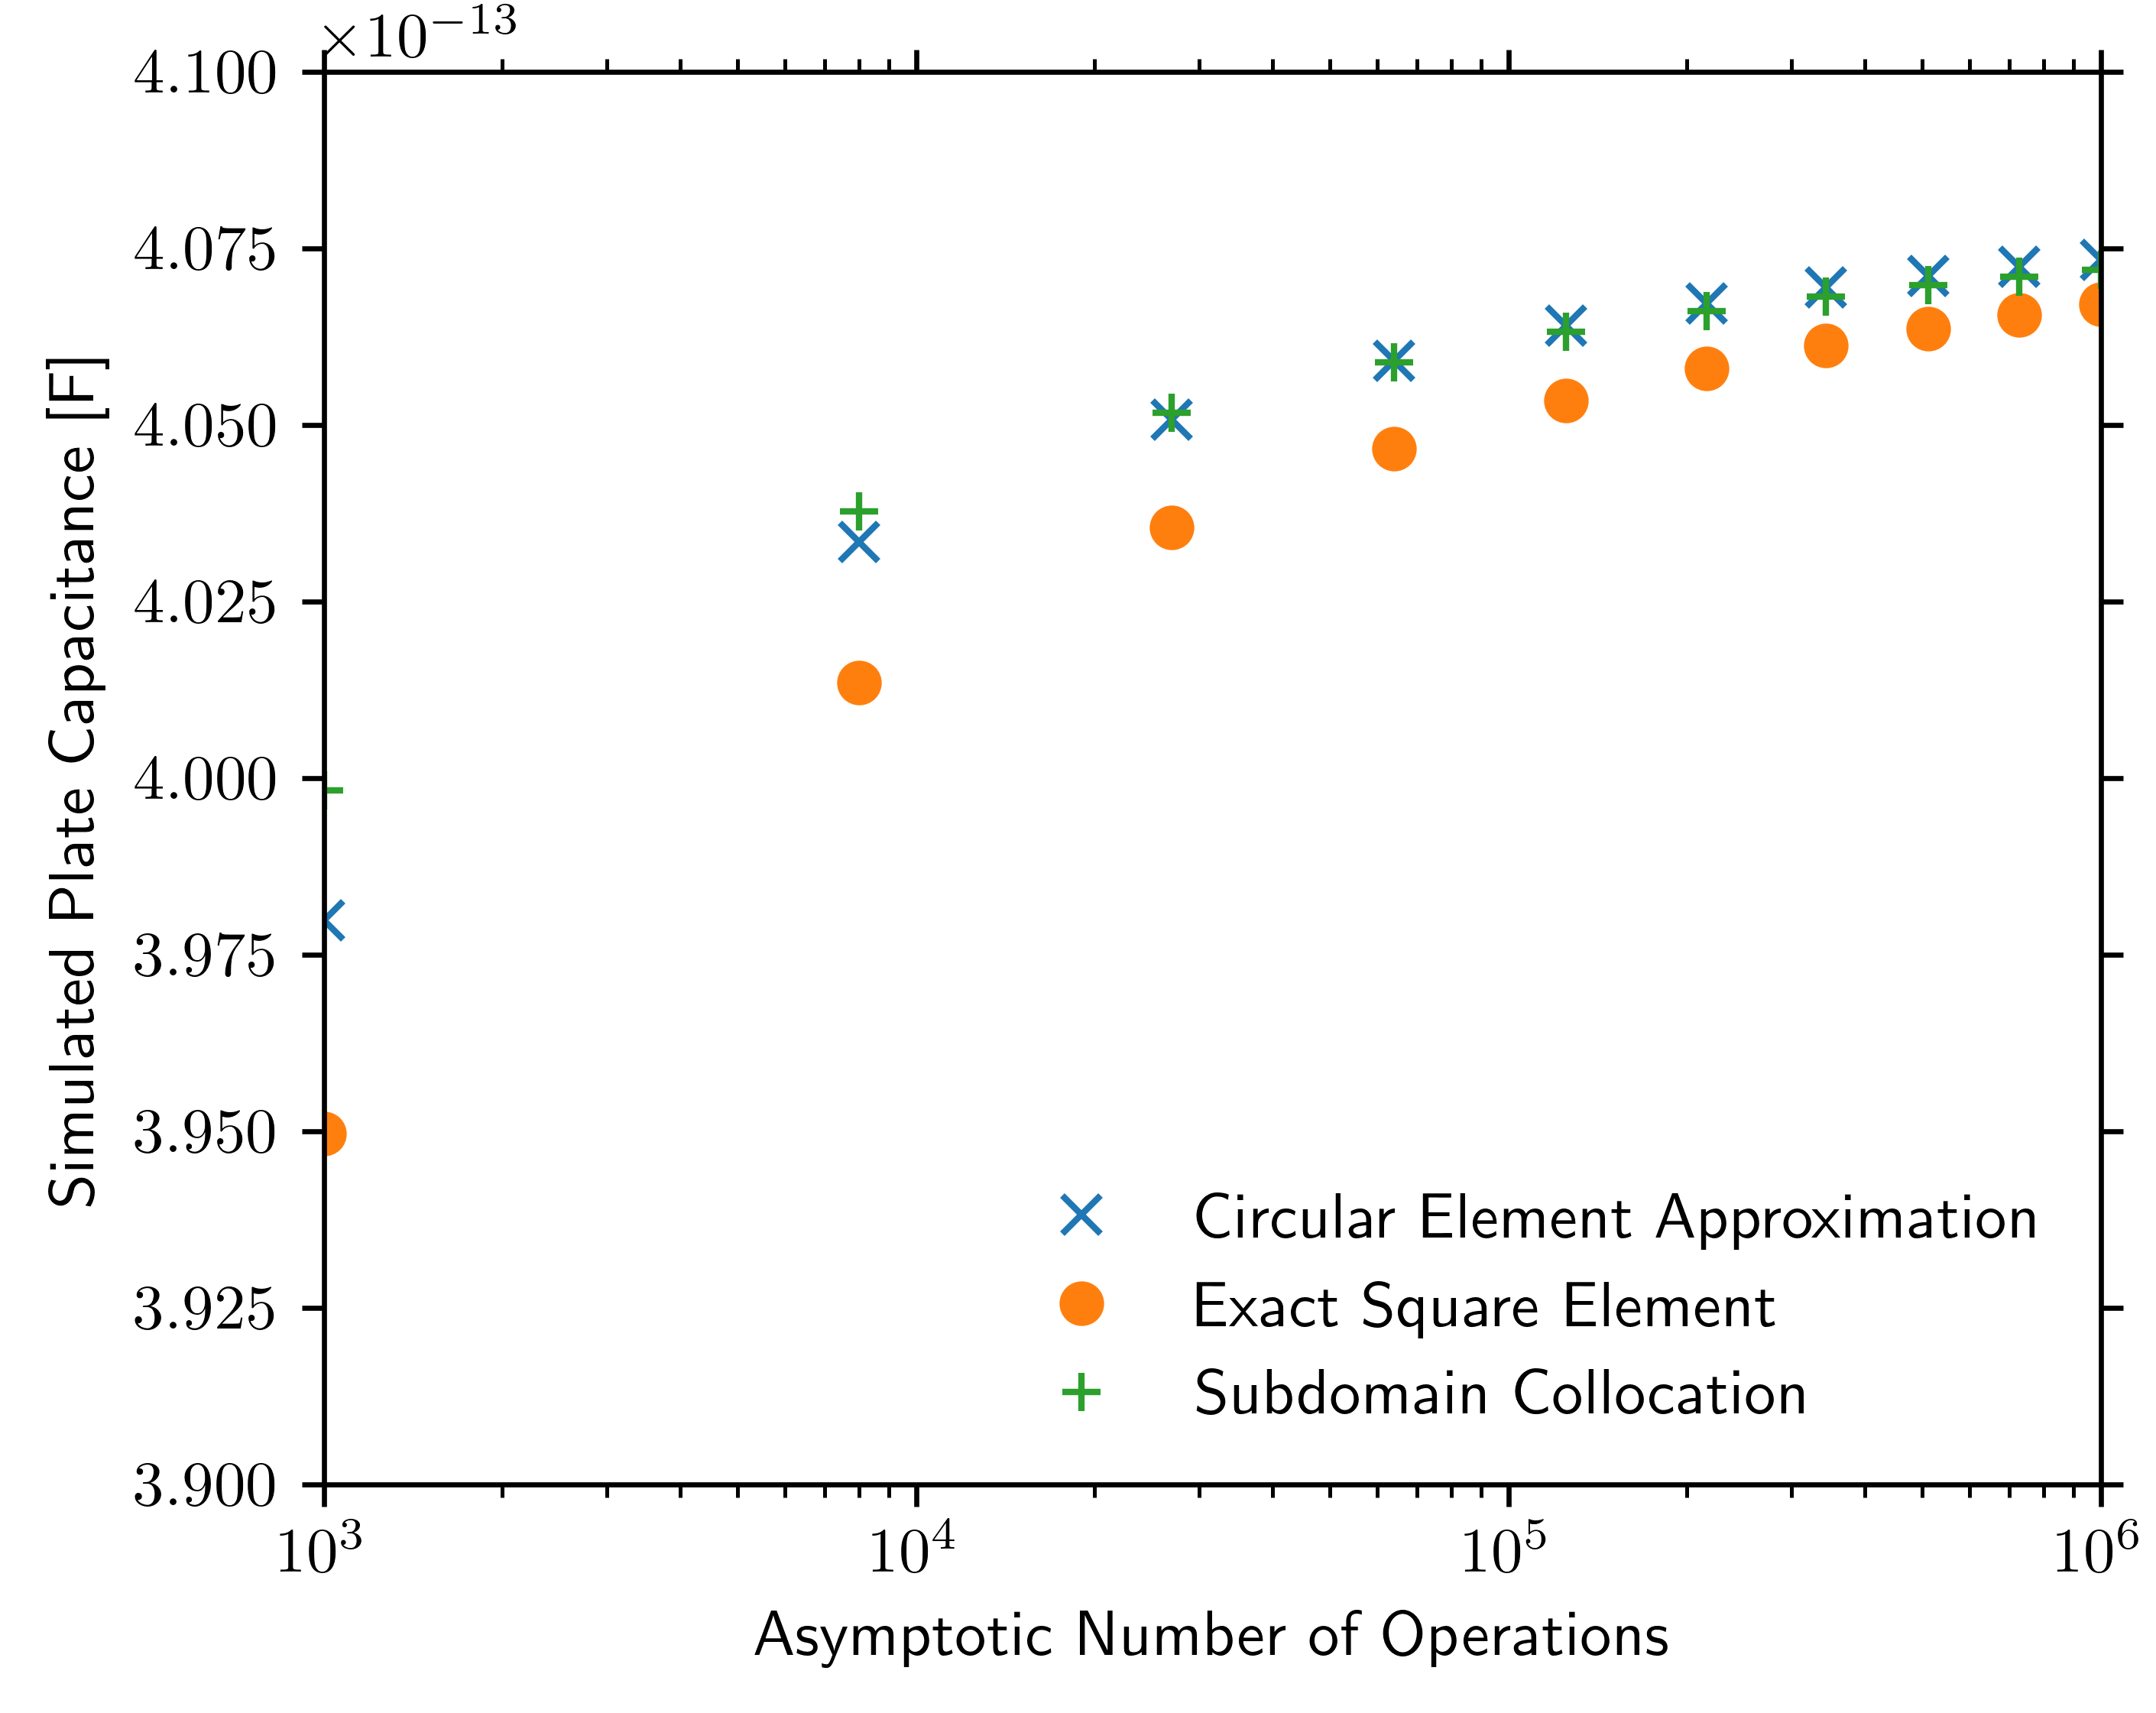
\includegraphics[width=\linewidth]{conv.png} 
	\caption{Example of caption text.}
	\label{fig:convergence}
\end{figure}